\documentclass{article}

\usepackage{fullpage}
\usepackage{amsmath}
\usepackage{amsfonts}
\usepackage{graphicx}
\usepackage{algorithmic}
\usepackage{xcolor}
\usepackage{framed}

\definecolor{dark_red}{rgb}{0.5,0.0,0.0}

\newcommand{\abs}[1]{\left|#1\right|}
\newcommand{\rowvec}[3]{\left\langle #1, #2, #3 \right\rangle}
\newcommand{\colvec}[3]{\begin{bmatrix} #1 \\ #2 \\ #3 \end{bmatrix}}
\newcommand{\at}[1]{\left. #1 \right|}
\newcommand{\diff}[2]{\frac{d #1}{d #2}}
\newcommand{\partdiff}[2]{\frac{\partial #1}{\partial #2}}
\newcommand{\mvec}[1]{\overrightarrow{\mathbf{#1}}}
\newcommand{\pvec}[1]{\overrightarrow{#1}}
\newcommand{\dr}[1]{\textcolor{dark_red}{#1}}



\title{Multi-variable Functions}
\date{}

\begin{document}

\maketitle



%%%%%%%%%%%%%%%%%%%%% QUESTION 1
\section*{Question 1:}

Draw the domains of the following multi-variable functions. For curves, use solid lines to include the curve as part of the domain, and use dashed lines to exclude the curve from the domain.

\begin{itemize}
\item \(f(x,y) = \frac{\sqrt{-x^2 + 4x}}{\sqrt{9 - x^2 - y^2}}\)
\item \(f(x,y) = \ln(x + y - x^2)\)
\item \(f(x,y) = \frac{\ln(x)}{xy + 2x - 3y - 6}\)
\end{itemize}

\vspace{0.5cm}

\dr{\bf Solution:}

\vspace{0.5cm}

\dr{For \(f(x,y) = \frac{\sqrt{-x^2 + 4x}}{\sqrt{9 - x^2 - y^2}}\), the required conditions on the input pair are \(-x^2 + 4x \geq 0\) so the numerator is real valued, and \(9 - x^2 - y^2 > 0\) so the denominator is both real valued and nonzero.}

\dr{The condition \(-x^2 + 4x \geq 0\) is equivalent to \(x(x-4) \leq 0 \iff (0 \leq x) \;\text{and}\; (x \leq 4)\)} 

\dr{The condition \(9 - x^2 - y^2 > 0\) is equivalent to \(\sqrt{x^2 + y^2} < 3\)}

\dr{The domain can then be drawn from the conditions \((0 \leq x) \;\text{and}\; (x \leq 4) \;\text{and}\; \sqrt{x^2 + y^2} < 3\):}


\includegraphics[width = 5cm]{Test_bench_part_2b_images/Question_1_part_1}

\dr{For \(f(x,y) = \ln(x + y - x^2)\), the required condition on the input pair is \(x + y - x^2 > 0\) so that \(\ln\) returns a real value. \(x + y - x^2 > 0\) is equivalent to \(y > x^2 - x\).} 

\dr{The domain can be drawn from the condition \(y > x^2 - x\):}


\includegraphics[width = 5cm]{Test_bench_part_2b_images/Question_1_part_2}

\dr{For \(f(x,y) = \frac{\ln(x)}{xy + 2x - 3y - 6}\), the required conditions on the input pair are \(x > 0\) so the numerator is real valued, and \(xy + 2x - 3y - 6 \neq 0\) so the denominator is nonzero.} 

\dr{The condition \(xy + 2x - 3y - 6 \neq 0\) is equivalent to \((x - 3)(y + 2) \neq 0 \iff (x \neq 3) \;\text{and}\; (y \neq -2)\)}

\dr{The domain can then be drawn from the conditions \((x > 0) \;\text{and}\; (x \neq 3) \;\text{and}\; (y \neq -2)\):}

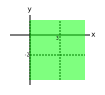
\includegraphics[width = 6cm]{Test_bench_part_2b_images/Question_1_part_3}

\vspace{0.5cm}


%%%%%%%%%%%%%%%%%%%%% QUESTION 2
\section*{Question 2:}

Compute the following limits:

\begin{itemize}
\item \(\lim_{t \to -1} \colvec{\sqrt{t + 3}}{\frac{t^2}{t+2}}{\ln(t + 5)}\)
\item \(\lim_{(x,y) \to (-1,-2)} \frac{\sqrt{x+y+5}}{x+y+4}\)
\end{itemize}

\vspace{0.5cm}

\dr{\bf Solution:}

\vspace{0.5cm}

\dr{For \(\colvec{\sqrt{t + 3}}{\frac{t^2}{t+2}}{\ln(t + 5)}\), there are no discontinuous singularities at \(t = -1\). Therefore \(\lim_{t \to -1} \colvec{\sqrt{t + 3}}{\frac{t^2}{t+2}}{\ln(t + 5)} = \colvec{\sqrt{-1 + 3}}{\frac{(-1)^2}{-1+2}}{\ln(-1 + 5)} = \colvec{\sqrt{2}}{1}{\ln(4)}\)}

\vspace{0.5cm}

\dr{For \(\frac{\sqrt{x+y+5}}{x+y+4}\), there are no discontinuous singularities at \((x,y) = (-1,-2)\). Therefore \(\lim_{(x,y) \to (-1,-2)} \frac{\sqrt{x+y+5}}{x+y+4} = \frac{\sqrt{(-1)+(-2)+5}}{(-1)+(-2)+4} = \sqrt{2}\)}


%%%%%%%%%%%%%%%%%%%%% QUESTION 3
\section*{Question 3:}

Define the two-variable function \(f(x,y) = \frac{xy}{x^2 + y^2}\).

%%%%%%%%%%%%%%%%%%%%% QUESTION 3A
\subsection*{part 3a:}

Compute the following partial derivatives:
\[\frac{\partial f}{\partial x} \quad \frac{\partial f}{\partial y} \quad \frac{\partial^2 f}{\partial x^2} \quad \frac{\partial^2 f}{\partial y^2} \quad \frac{\partial^2 f}{\partial y \partial x}\] 

\vspace{0.5cm}

\dr{\bf Solution:}

\vspace{0.5cm}

\dr{Using the quotient rule, the first order partial derivatives can be computed:
\[\partdiff{f}{x} = \frac{(y)(x^2 + y^2) - (xy)(2x)}{(x^2 + y^2)^2} = \frac{-x^2y + y^3}{(x^2 + y^2)^2}\] 
and
\[\partdiff{f}{y} = \frac{(x)(x^2 + y^2) - (xy)(2y)}{(x^2 + y^2)^2} = \frac{x^3 - xy^2}{(x^2 + y^2)^2}\]
}

\dr{Further using the quotient rule, the second order partial derivatives can be computed:
\begin{align*}
\frac{\partial^2 f}{\partial x^2} = & \frac{(-2xy)(x^2 + y^2)^2 - (-x^2y + y^3)(2(x^2 + y^2)(2x))}{(x^2 + y^2)^4} \\
= & \frac{-2xy(x^2 + y^2) - 4x(-x^2y + y^3)}{(x^2 + y^2)^3}    
= \frac{2x^3y - 6xy^3}{(x^2 + y^2)^3}
\end{align*}
\begin{align*}
\frac{\partial^2 f}{\partial y^2} = & \frac{(-2xy)(x^2 + y^2)^2 - (x^3 - xy^2)(2(x^2 + y^2)(2y))}{(x^2 + y^2)^4} \\
= & \frac{-2xy(x^2 + y^2) - 4y(x^3 - xy^2)}{(x^2 + y^2)^3} 
= \frac{-6x^3y + 2xy^3}{(x^2 + y^2)^3}
\end{align*}
\begin{align*}
\frac{\partial^2 f}{\partial y \partial x} = & \frac{(-x^2 + 3y^2)(x^2 + y^2)^2 - (-x^2y + y^3)(2(x^2 + y^2)(2y))}{(x^2 + y^2)^4} \\
= & \frac{(-x^2 + 3y^2)(x^2 + y^2) - 4y(-x^2y + y^3)}{(x^2 + y^2)^3} \\
= & \frac{(-x^4 + 2x^2y^2 + 3y^4) + (4x^2y^2 - 4y^4)}{(x^2 + y^2)^3} 
= \frac{-x^4 + 6x^2y^2 - y^4}{(x^2 + y^2)^3}
\end{align*}
}

%%%%%%%%%%%%%%%%%%%%% QUESTION 3B
\subsection*{part 3b:}

Compute the gradient \(\nabla f\) at the point \((x_0,y_0) = (3,1)\). Compute the equation of the tangent plane to the surface \(z = f(x,y)\) that passes through the point \((x_0,y_0,f(x_0,y_0))\). Given a direction of \(\mathbf{v} = \langle 3, -4 \rangle\), what is the ``directional derivative" of \(f(x,y)\) at \((x_0, y_0)\) in the direction of \(\mathbf{v}\)?

\vspace{0.5cm}

\dr{\bf Solution:}

\vspace{0.5cm}

\dr{\[\at{\nabla f}_{(3,1)} = \left\langle \frac{-9 + 1}{(9 + 1)^2} , \frac{27 - 3}{(9 + 1)^2} \right\rangle = \left\langle \frac{-8}{100} , \frac{24}{100} \right\rangle = \left\langle \frac{-2}{25} , \frac{6}{25} \right\rangle\]}

\dr{From \(f(3,1) = \frac{3}{9 + 1} = \frac{3}{10}\) and \(\at{\nabla f}_{(3,1)} = \left\langle \frac{-2}{25} , \frac{6}{25} \right\rangle\), the tangent plane that passes through the point \((3,1,3/10)\) is 
\[z = \frac{3}{10} + \frac{-2}{25}(x - 3) + \frac{6}{25}(y - 1) \iff z = -\frac{2}{25}x + \frac{6}{25}y + \frac{3}{10}\]}

\dr{A unit vector that shares the direction of \(\mathbf{v}\) is \(\mathbf{u} = \frac{\mathbf{v}}{\abs{\mathbf{v}}} = \frac{1}{\sqrt{9 + 16}}\langle 3, -4 \rangle = \left\langle \frac{3}{5}, -\frac{4}{5} \right\rangle\). The directional derivative at \((3, 1)\) in the direction of \(\mathbf{v}\) is \(\mathbf{u} \cdot (\at{\nabla f}_{(3,1)}) = \frac{3}{5}\cdot\frac{-2}{25} + (-\frac{4}{5})\cdot\frac{6}{25} = \frac{-6}{125} + \frac{-24}{125} = \frac{-30}{125} = \frac{-6}{25}\).}



%%%%%%%%%%%%%%%%%%%%% QUESTION 4
\section*{Question 4:}

\begin{center}
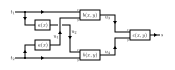
\includegraphics[width = \textwidth]{chain_rule_XOR_circuit}
\end{center}

In the flow-chart (arithmetic circuit) above, the output quantity \(s\) is being computed from input quantities \(t_1\) and \(t_2\). There are the internal variables \(u_1\), \(u_2\), \(u_3\), and \(u_4\).

%%%%%%%%%%%%%%%%%%%%% QUESTION 4A
\subsection*{part 4a:}

Build expressions for \(u_1\), \(u_2\), \(u_3\), \(u_4\), and \(s\) from the input parameters \(t_1\) and \(t_2\), and the functions \(a(x)\), \(b(x,y)\), and \(c(x,y)\).

\vspace{0.5cm}

\dr{\bf Solution:}

\dr{\begin{itemize}
\item \(u_1 = a(t_2)\)
\item \(u_2 = a(t_1)\) 
\item \(u_3 = b(t_1,u_1) = b(t_1,a(t_2))\)
\item \(u_4 = b(u_2,t_2) = b(a(t_1),t_2)\)
\item \(s = c(u_3,u_4) = c(b(t_1,a(t_2)),b(a(t_1),t_2))\)
\end{itemize}}



%%%%%%%%%%%%%%%%%%%%% QUESTION 4B
\subsection*{part 4b:}

Without any knowledge of \(a(x)\), \(b(x,y)\), or \(c(x,y)\), derive expressions for the following partial derivatives: \(\partdiff{u_1}{t_1}\), \(\partdiff{u_1}{t_2}\), \(\partdiff{u_2}{t_1}\), and \(\partdiff{u_2}{t_2}\).

Derive expressions for the following partial derivatives: \(\partdiff{u_3}{t_1}\), \(\partdiff{u_3}{t_2}\), \(\partdiff{u_4}{t_1}\), and \(\partdiff{u_4}{t_2}\) in terms of the partial derivatives computed previously.

Derive expressions for the following partial derivatives: \(\partdiff{s}{t_1}\), and \(\partdiff{s}{t_2}\) in terms of the partial derivatives computed previously.

\vspace{0.5cm}

\dr{\bf Solution:}

\vspace{0.5cm}

\dr{~~\(u_1\) is the output of function \(a\) with input \(t_2\) so \(\partdiff{u_1}{t_1} = \at{\diff{a}{x}}_{t_2}(0) = 0\) and \(\partdiff{u_1}{t_2} = \at{\diff{a}{x}}_{t_2}(1) = \at{\diff{a}{x}}_{t_2}\)}

\dr{~~\(u_2\) is the output of function \(a\) with input \(t_1\) so \(\partdiff{u_2}{t_1} = \at{\diff{a}{x}}_{t_1}(1) = \at{\diff{a}{x}}_{t_1}\) and \(\partdiff{u_2}{t_2} = \at{\diff{a}{x}}_{t_1}(0) = 0\)}

\dr{~~\(u_3\) is the output of function \(b\) with respective inputs \(t_1\) and \(u_1\) so 
\[\partdiff{u_3}{t_1} = \at{\partdiff{b}{x}}_{(t_1,u_1)}(1) + \at{\partdiff{b}{y}}_{(t_1,u_1)}\cdot\partdiff{u_1}{t_1} = \at{\partdiff{b}{x}}_{(t_1,u_1)} + \at{\partdiff{b}{y}}_{(t_1,u_1)}\cdot\partdiff{u_1}{t_1}\] and 
\[\partdiff{u_3}{t_2} = \at{\partdiff{b}{x}}_{(t_1,u_1)}(0) + \at{\partdiff{b}{y}}_{(t_1,u_1)}\cdot\partdiff{u_1}{t_2} = \at{\partdiff{b}{y}}_{(t_1,u_1)}\cdot\partdiff{u_1}{t_2}\]}

\dr{~~\(u_4\) is the output of function \(b\) with respective inputs \(u_2\) and \(t_2\) so 
\[\frac{\partial u_4}{\partial t_1} = \at{\frac{\partial b}{\partial x}}_{(u_2,t_2)}\cdot\frac{\partial u_2}{\partial t_1} + \at{\frac{\partial b}{\partial y}}_{(u_2,t_2)}(0) = \at{\frac{\partial b}{\partial x}}_{(u_2,t_2)}\cdot\frac{\partial u_2}{\partial t_1}\] and 
\[\frac{\partial u_4}{\partial t_2} = \at{\frac{\partial b}{\partial x}}_{(u_2,t_2)}\cdot\frac{\partial u_2}{\partial t_2} + \at{\frac{\partial b}{\partial y}}_{(u_2,t_2)}(1) = \at{\frac{\partial b}{\partial x}}_{(u_2,t_2)}\cdot\frac{\partial u_2}{\partial t_2} + \at{\frac{\partial b}{\partial y}}_{(u_2,t_2)}\]}

\dr{~~\(s\) is the output of function \(c\) with respective inputs \(u_3\) and \(u_4\) so 
\[\frac{\partial s}{\partial t_1} = \at{\frac{\partial c}{\partial x}}_{(u_3,u_4)}\cdot\frac{\partial u_3}{\partial t_1} + \at{\frac{\partial c}{\partial y}}_{(u_3,u_4)}\cdot\frac{\partial u_4}{\partial t_1}\] and 
\[\frac{\partial s}{\partial t_2} = \at{\frac{\partial c}{\partial x}}_{(u_3,u_4)}\cdot\frac{\partial u_3}{\partial t_2} + \at{\frac{\partial c}{\partial y}}_{(u_3,u_4)}\cdot\frac{\partial u_4}{\partial t_2}\]}

\dr{In summary: \begin{itemize}
\item 
\(\partdiff{u_1}{t_1} = 0\) and 
\(\partdiff{u_1}{t_2} = \at{\diff{a}{x}}_{t_2}\)
\item 
\(\partdiff{u_2}{t_1} = \at{\diff{a}{x}}_{t_1}\) and 
\(\partdiff{u_2}{t_2} = 0\)
\item 
\(\partdiff{u_3}{t_1} = \at{\partdiff{b}{x}}_{(t_1,u_1)} + \at{\partdiff{b}{y}}_{(t_1,u_1)}\cdot\partdiff{u_1}{t_1}\) and 
\(\partdiff{u_3}{t_2} = \at{\partdiff{b}{y}}_{(t_1,u_1)}\cdot\partdiff{u_1}{t_2}\)
\item 
\(\partdiff{u_4}{t_1} = \at{\partdiff{b}{x}}_{(u_2,t_2)}\cdot\partdiff{u_2}{t_1}\) and 
\(\partdiff{u_4}{t_2} = \at{\partdiff{b}{x}}_{(u_2,t_2)}\cdot\partdiff{u_2}{t_2} + \at{\partdiff{b}{y}}_{(u_2,t_2)}\)
\item
\(\partdiff{s}{t_1} = \at{\partdiff{c}{x}}_{(u_3,u_4)}\cdot\partdiff{u_3}{t_1} + \at{\partdiff{c}{y}}_{(u_3,u_4)}\cdot\partdiff{u_4}{t_1}\) and 
\(\partdiff{s}{t_2} = \at{\partdiff{c}{x}}_{(u_3,u_4)}\cdot\partdiff{u_3}{t_2} + \at{\partdiff{c}{y}}_{(u_3,u_4)}\cdot\partdiff{u_4}{t_2}\)
\end{itemize}}

%%%%%%%%%%%%%%%%%%%%% QUESTION 4C
\subsection*{part 4c:}

Now let \(a(x) = 1 - x\), \(b(x,y) = xy\), and \(c(x,y) = x + y - xy\). Compute all first-order derivatives: \(\frac{da}{dx}\), \(\frac{\partial b}{\partial x}\), \(\frac{\partial b}{\partial y}\), \(\frac{\partial c}{\partial x}\), and \(\frac{\partial c}{\partial y}\).

\vspace{0.5cm}

\dr{\bf Solution:}

\vspace{0.5cm}

\dr{\begin{itemize}
\item \(\frac{da}{dx} = -1\)
\item \(\frac{\partial b}{\partial x} = y\) and \(\frac{\partial b}{\partial y} = x\)
\item \(\frac{\partial c}{\partial x} = 1 - y\) and \(\frac{\partial c}{\partial y} = 1 - x\)
\end{itemize}}

\vspace{0.5cm}



%%%%%%%%%%%%%%%%%%%%% QUESTION 4D
\subsection*{part 4d:}

From the results of the previous sections, compute at \((t_1, t_2) = (3/4, 1/4)\) the output \(s\), as well as the partial derivatives \(\frac{\partial s}{\partial t_1}\) and \(\frac{\partial s}{\partial t_2}\).

\vspace{0.5cm}

\dr{\bf Solution:}

\vspace{0.5cm}

\dr{From \(t_1 = 3/4\) and \(t_2 = 1/4\), \(u_1 = a(t_2) = 3/4\), \(u_2 = a(t_1) = 1/4\), \(u_3 = b(t_1,u_1) = (3/4)(3/4) = 9/16\), \(u_4 = b(u_2,t_2) = (1/4)(1/4) = 1/16\), and \(s = c(u_3,u_4) = 9/16 + 1/16 - (9/16)(1/16) = 10/16 - 9/256 = (160 - 9)/256 = 151/256\).}

\vspace{0.4cm}

\dr{\(\partdiff{u_1}{t_1} = 0\) and \(\partdiff{u_1}{t_2} = \at{\diff{a}{x}}_{1/4} = -1\)}

\vspace{0.4cm}

\dr{\(\partdiff{u_2}{t_1} = \at{\diff{a}{x}}_{3/4} = -1\) and \(\partdiff{u_2}{t_2} = 0\)}

\vspace{0.4cm}

\dr{\(\partdiff{u_3}{t_1} = \at{\partdiff{b}{x}}_{(3/4,3/4)} + \at{\partdiff{b}{y}}_{(3/4,3/4)}\cdot\partdiff{u_1}{t_1} = 3/4 + (3/4)(0) = 3/4\) \\ and 
\(\partdiff{u_3}{t_2} = \at{\frac{\partial b}{\partial y}}_{(3/4,3/4)}\cdot\frac{\partial u_1}{\partial t_2} = (3/4)(-1) = -3/4\)}

\vspace{0.4cm}

\dr{\(\partdiff{u_4}{t_1} = \at{\partdiff{b}{x}}_{(1/4,1/4)}\cdot\partdiff{u_2}{t_1} = (1/4)(-1) = -1/4\) \\ and 
\(\partdiff{u_4}{t_2} = \at{\partdiff{b}{x}}_{(1/4,1/4)}\cdot\partdiff{u_2}{t_2} + \at{\partdiff{b}{y}}_{(1/4,1/4)} = (1/4)(0) + 1/4 = 1/4\)}

\vspace{0.4cm}

\dr{\(\partdiff{s}{t_1} = \at{\partdiff{c}{x}}_{(9/16,1/16)}\cdot\partdiff{u_3}{t_1} + \at{\partdiff{c}{y}}_{(9/16,1/16)}\cdot\partdiff{u_4}{t_1} = (1 - 1/16)(3/4) + (1 - 9/16)(-1/4) = (15/16)(3/4) + (7/16)(-1/4) = (45 - 7)/64 = 38/64 = 19/32\) \\ and 
\(\partdiff{s}{t_2} = \at{\partdiff{c}{x}}_{(9/16,1/16)}\cdot\partdiff{u_3}{t_2} + \at{\partdiff{c}{y}}_{(9/16,1/16)}\cdot\partdiff{u_4}{t_2} = (1 - 1/16)(-3/4) + (1 - 9/16)(1/4) = (15/16)(-3/4) + (7/16)(1/4) = (-45 + 7)/64 = -38/64 = -19/32\)}

\vspace{0.4cm}

\dr{Therefore \(s = 151/256\), \(\partdiff{s}{t_1} = 19/32\) and \(\partdiff{s}{t_2} = -19/32\).}



%%%%%%%%%%%%%%%%%%%%% QUESTION 5
\section*{Question 5:}

For each of the following two variable functions \(f(x,y)\), find and classify all of the critical points:

\begin{itemize}
\item \(f(x,y) = -11x^2 + 6xy - 19y^2 + 78x - 94y - 211\)
\item \(f(x,y) = \frac{1}{3}x^3 - \frac{7}{18}x^2 - \frac{2}{3}xy + y^2 - \frac{10}{9}x - \frac{8}{3}y + \frac{16}{9}\)
\item \(f(x,y) = \frac{1}{3}x^3 + \frac{7}{16}x^2 - \frac{3}{2}xy - y^2 - \frac{3}{8}x + \frac{7}{2}y - \frac{49}{16}\)
\item \(f(x,y) = \frac{1}{3}y^3 - x^2 - \frac{3}{2}xy + \frac{7}{16}y^2 - \frac{5}{2}x - \frac{39}{8}y - \frac{25}{16}\)
\item \(f(x,y) = \frac{5}{4}x^4 - \frac{1}{3}x^3 - 2x^2y - 2x^2 + y^2 + 4x\)
\end{itemize}

\vspace{0.5cm}

\dr{\bf Solution:}

\vspace{0.5cm}

%PART 5,1
\dr{For \(f(x,y) = -11x^2 + 6xy - 19y^2 + 78x - 94y - 211\), the first and second order partial derivatives are: 
\(\partdiff{f}{x} = -22x + 6y + 78\); \(\partdiff{f}{y} = 6x - 38y - 94\); \(\frac{\partial^2 f}{\partial x^2} = -22\); \(\frac{\partial^2 f}{\partial y^2} = -38\); and \(\frac{\partial^2 f}{\partial y \partial x} = 6\)}

\dr{Finding the critical points requires solving the system: \(\left\{\begin{array}{c} \partial f/\partial x = 0 \\ \partial f/\partial y = 0 \end{array}\right. \iff \left\{\begin{array}{c} -22x + 6y + 78 = 0 \\ 6x - 38y - 94 = 0 \end{array}\right.\)}

\dr{The first equation gives \(y = (11/3)x - 13\). Substituting into the second equation gives \\ \(6x + ((-418/3)x + 494) - 94 = 0 \iff (-400/3)x + 400 = 0 \iff x = 3\). This gives \(y = -2\).}

\dr{There is hence only one critical point \((x_c, y_c) = (3, -2)\).}

\dr{The discriminant at \((3, -2)\) is \(\Delta = (-22)(-38) - (6)^2 = 836 - 36 = 800 > 0\). Since both \(\frac{\partial^2 f}{\partial x^2}\) and \(\frac{\partial^2 f}{\partial y^2}\) are negative, \((3, -2)\) is a local maximum.}

\vspace{1cm}

%PART 5,2
\dr{For \(f(x,y) = \frac{1}{3}x^3 - \frac{7}{18}x^2 - \frac{2}{3}xy + y^2 - \frac{10}{9}x - \frac{8}{3}y + \frac{16}{9}\), the first and second order partial derivatives are: 
\(\partdiff{f}{x} = x^2 - \frac{7}{9}x - \frac{2}{3}y - \frac{10}{9}\); \(\partdiff{f}{y} = -\frac{2}{3}x + 2y - \frac{8}{3}\); \(\frac{\partial^2 f}{\partial x^2} = 2x - \frac{7}{9}\); \(\frac{\partial^2 f}{\partial y^2} = 2\); and \(\frac{\partial^2 f}{\partial y \partial x} = -\frac{2}{3}\)}

\dr{Finding the critical points requires solving the system: \(\left\{\begin{array}{c} \partial f/\partial x = 0 \\ \partial f/\partial y = 0 \end{array}\right. \iff \left\{\begin{array}{c} x^2 - \frac{7}{9}x - \frac{2}{3}y - \frac{10}{9} = 0 \\ -\frac{2}{3}x + 2y - \frac{8}{3} = 0 \end{array}\right.\)}

\dr{The first equation gives \(y = \frac{3}{2}x^2 - \frac{7}{6}x - \frac{5}{3}\). Substituting into the second equation gives \\ \(-\frac{2}{3}x + (3x^2 -\frac{7}{3}x - \frac{10}{3}) - \frac{8}{3} = 0 \iff 3x^2 - 3x - 6 = 0 \iff x^2 - x - 2 = 0 \iff (x + 1)(x - 2) = 0 \iff x = -1,2\). \(x = -1\) gives \(y = \frac{3}{2} + \frac{7}{6} - \frac{5}{3} = \frac{9 + 7 - 10}{6} = 1\). \(x = 2\) gives \(y = 6 - \frac{7}{3} - \frac{5}{3} = 6 - \frac{12}{3} = 2\).}

\dr{There are two critical points \((x_c, y_c) = (-1,1); (2,2)\).}

\dr{The discriminant at \((-1,1)\) is \(\Delta = (-\frac{25}{9})(2) - (-\frac{2}{3})^2 = -\frac{50}{9} - \frac{4}{9} = -6 < 0\). Hence \((-1,1)\) is a saddle point.}

\dr{The discriminant at \((2,2)\) is \(\Delta = (\frac{29}{9})(2) - (-\frac{2}{3})^2 = \frac{58}{9} - \frac{4}{9} = 6 > 0\). Since both \(\frac{\partial^2 f}{\partial x^2}\) and \(\frac{\partial^2 f}{\partial y^2}\) are positive, \((2,2)\) is a local minimum.}

\vspace{1cm}

%PART 5,3
\dr{For \(f(x,y) = \frac{1}{3}x^3 + \frac{7}{16}x^2 - \frac{3}{2}xy - y^2 - \frac{3}{8}x + \frac{7}{2}y - \frac{49}{16}\), the first and second order partial derivatives are: 
\(\partdiff{f}{x} = x^2 + \frac{7}{8}x - \frac{3}{2}y - \frac{3}{8}\); \(\partdiff{f}{y} = -\frac{3}{2}x - 2y + \frac{7}{2}\); \(\frac{\partial^2 f}{\partial x^2} = 2x + \frac{7}{8}\); \(\frac{\partial^2 f}{\partial y^2} = -2\); and \(\frac{\partial^2 f}{\partial y \partial x} = -\frac{3}{2}\)}

\dr{Finding the critical points requires solving the system: \(\left\{\begin{array}{c} \partial f/\partial x = 0 \\ \partial f/\partial y = 0 \end{array}\right. \iff \left\{\begin{array}{c} x^2 + \frac{7}{8}x - \frac{3}{2}y - \frac{3}{8} = 0 \\ -\frac{3}{2}x - 2y + \frac{7}{2} = 0 \end{array}\right.\)}

\dr{The first equation gives \(y = \frac{2}{3}x^2 + \frac{7}{12}x - \frac{1}{4}\). Substituting into the second equation gives \\ \(-\frac{3}{2}x + (-\frac{4}{3}x^2 -\frac{7}{6}x + \frac{1}{2}) + \frac{7}{2} = 0 \iff -\frac{4}{3}x^2 - \frac{16}{6}x + 4 = 0 \iff x^2 + 2x - 3 = 0 \iff (x + 3)(x - 1) = 0 \iff x = -3,1\). \(x = -3\) gives \(y = 6 - \frac{7}{4} - \frac{1}{4} = 6 - 2 = 4\). \(x = 1\) gives \(y = \frac{2}{3} + \frac{7}{12} - \frac{1}{4} = \frac{8 + 7 - 3}{12} = 1\).}

\dr{There are two critical points \((x_c, y_c) = (-3,4); (1,1)\).}

\dr{The discriminant at \((-3,4)\) is \(\Delta = (-\frac{41}{8})(-2) - (-\frac{3}{2})^2 = \frac{41}{4} - \frac{9}{4} = 8 > 0\). Since both \(\frac{\partial^2 f}{\partial x^2}\) and \(\frac{\partial^2 f}{\partial y^2}\) are negative, \((-3,4)\) is a local maximum.}

\dr{The discriminant at \((1,1)\) is \(\Delta = (\frac{23}{8})(-2) - (-\frac{3}{2})^2 = -\frac{23}{4} - \frac{9}{4} = \frac{-32}{4} = -8 < 0\). Hence \((1,1)\) is a saddle point.}

\vspace{1cm}

%PART 5,4
\dr{For \(f(x,y) = \frac{1}{3}y^3 - x^2 - \frac{3}{2}xy + \frac{7}{16}y^2 - \frac{5}{2}x - \frac{39}{8}y - \frac{25}{16}\), the first and second order partial derivatives are: 
\(\partdiff{f}{x} = -2x - \frac{3}{2}y - \frac{5}{2}\); \(\partdiff{f}{y} = y^2 - \frac{3}{2}x + \frac{7}{8}y - \frac{39}{8}\); \(\frac{\partial^2 f}{\partial x^2} = -2\); \(\frac{\partial^2 f}{\partial y^2} = 2y + \frac{7}{8}\); and \(\frac{\partial^2 f}{\partial y \partial x} = -\frac{3}{2}\)}

\dr{Finding the critical points requires solving the system: \(\left\{\begin{array}{c} \partial f/\partial x = 0 \\ \partial f/\partial y = 0 \end{array}\right. \iff \left\{\begin{array}{c} -2x - \frac{3}{2}y - \frac{5}{2} = 0 \\ y^2 - \frac{3}{2}x + \frac{7}{8}y - \frac{39}{8} = 0 \end{array}\right.\)}

\dr{The first equation gives \(x = -\frac{5}{4} - \frac{3}{4}y\). Substituting into the second equation gives \\ \(y^2 + (\frac{15}{8} + \frac{9}{8}y) + \frac{7}{8}y - \frac{39}{8} = 0 \iff y^2 + 2y - 3 \iff (y + 3)(y - 1) = 0 \iff y = -3,1\). \(y = -3\) gives \(x = 1\). \(y = 1\) gives \(x = -2\).}

\dr{There are two critical points \((x_c, y_c) = (1,-3); (-2,1)\).}

\dr{The discriminant at \((1,-3)\) is \(\Delta = (-2)(-\frac{41}{8}) - (-\frac{3}{2})^2 = \frac{41}{4} - \frac{9}{4} = 8 > 0\). Since both \(\frac{\partial^2 f}{\partial x^2}\) and \(\frac{\partial^2 f}{\partial y^2}\) are negative, \((1,-3)\) is a local maximum.}

\dr{The discriminant at \((-2,1)\) is \(\Delta = (-2)(\frac{23}{8}) - (-\frac{3}{2})^2 = -\frac{23}{4} - \frac{9}{4} = -8 < 0\). Hence \((-2,1)\) is a saddle point.}

\vspace{1cm}

%PART 5,5
\dr{For \(f(x,y) = \frac{5}{4}x^4 - \frac{1}{3}x^3 - 2x^2y - 2x^2 + y^2 + 4x\), the first and second order partial derivatives are: 
\(\partdiff{f}{x} = 5x^3 - x^2 - 4xy - 4x + 4\); \(\partdiff{f}{y} = -2x^2 + 2y\); \(\frac{\partial^2 f}{\partial x^2} = 15x^2 - 2x - 4y - 4\); \(\frac{\partial^2 f}{\partial y^2} = 2\); and \(\frac{\partial^2 f}{\partial y \partial x} = -4x\)}

\dr{Finding the critical points requires solving the system: \(\left\{\begin{array}{c} \partial f/\partial x = 0 \\ \partial f/\partial y = 0 \end{array}\right. \iff \left\{\begin{array}{c} 5x^3 - x^2 - 4xy - 4x + 4 = 0 \\ -2x^2 + 2y = 0 \end{array}\right.\)}

\dr{The second equation gives \(y = x^2\). Substituting into the first equation gives \\ \(x^3 - x^2 - 4x + 4 = 0 \iff x^2(x-1) - 4(x-1) = 0 \iff (x-1)(x^2-4) = 0 \iff (x+2)(x-1)(x-2) = 0 \iff x = -2,1,2\). \(x = -2\) gives \(y = 4\). \(x = 1\) gives \(y = 1\). \(x = 2\) gives \(y = 4\).}

\dr{There are three critical points \((x_c, y_c) = (-2,4); (1,1); (2,4)\).}

\dr{The discriminant at \((-2,4)\) is \(\Delta = (44)(2) - (8)^2 = 88 - 64 = 24 > 0\). Since both \(\frac{\partial^2 f}{\partial x^2}\) and \(\frac{\partial^2 f}{\partial y^2}\) are positive, \((-2,4)\) is a local minimum.}

\dr{The discriminant at \((1,1)\) is \(\Delta = (5)(2) - (-4)^2 = 10 - 16 = -6 < 0\). Hence \((1,1)\) is a saddle point.}

\dr{The discriminant at \((2,4)\) is \(\Delta = (36)(2) - (-8)^2 = 72 - 64 = 8 > 0\). Since both \(\frac{\partial^2 f}{\partial x^2}\) and \(\frac{\partial^2 f}{\partial y^2}\) are positive, \((2,4)\) is a local minimum.}


\end{document}









